\documentclass{beamer}
\usepackage{tikz}
\usepackage{pgfplots}
\usepackage{mathtools}
\newcommand{\argmin}{\operatornamewithlimits{argmin}}

\usetikzlibrary{arrows,positioning} 
\tikzset{>=stealth',
    punkt/.style={rectangle, rounded corners, draw=black, very thick,
                    text width=6.5em, minimum height=2em, text centered},
    pil/.style={->, thick, shorten <=2pt, shorten >=2pt,}}

\beamertemplatenavigationsymbolsempty{}

\title{Optimization of a Distributed Storage Architecture under Uncertain
Demand}
\subtitle{A Study in Fast Flow Algorithms}
\date{March 20, 2015}

\author{Paul Beaujean\inst{*}\inst{\dag} \and \'Eric Gourdin\inst{\dag}}
\institute{\inst{*}ENSIIE-MPRO \and \inst{\dag}Orange Labs}

\begin{document}

\frame{\titlepage}

\begin{frame}
    \frametitle{Table of Contents}
    \tableofcontents{}
\end{frame}

\section{Context}
\subsection{The rise of IP video}
\begin{frame}
    \frametitle{Context: The rise of IP video}

    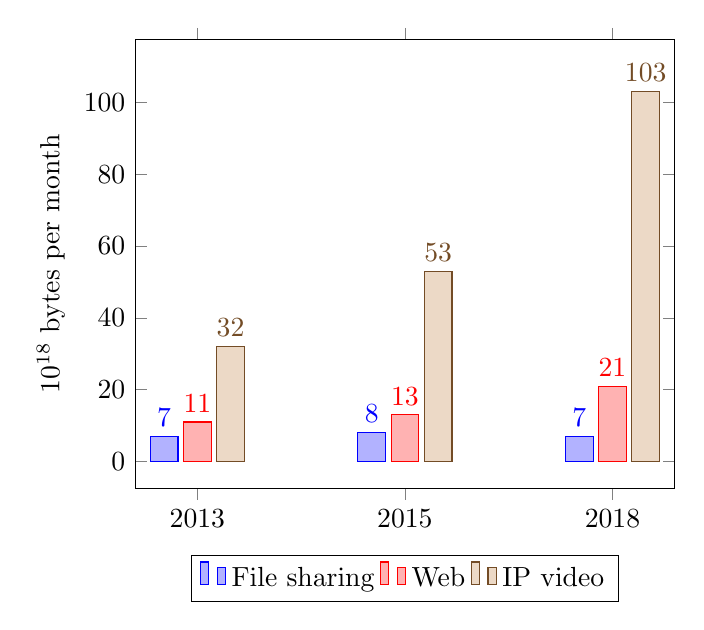
\begin{tikzpicture}
        \begin{axis}[
            ybar,
            enlargelimits=0.15,
            legend style={at={(0.5,-0.15)},
            anchor=north,legend columns=-1},
            ylabel={$10^{18}$ bytes per month},
            symbolic x coords={2013,2015,2018},
            xtick=data,
            nodes near coords,
            nodes near coords align={vertical},
            ]
            \addplot coordinates {(2013,7) (2015,8) (2018,7)};
            \addplot coordinates {(2013,11) (2015,13) (2018,21)};
            \addplot coordinates {(2013,32) (2015,53) (2018,103)};
            \legend{File sharing,Web,IP video}
        \end{axis}
    \end{tikzpicture}

    \begin{itemize}
        \item IP video: 80\% of all IP traffic by 2020.
    \end{itemize}
    \hfill\tiny{Source: CISCO Visual Networking Index 2014}

\end{frame}

\subsection{A solution: Content Delivery Network}
\begin{frame}
    \frametitle{Content Delivery Network}

    \begin{itemize}
        \item distributed storage architecture
        \item reduced upstream bandwidth consumption
        \item increased quality of service
    \end{itemize}
    \begin{figure}
    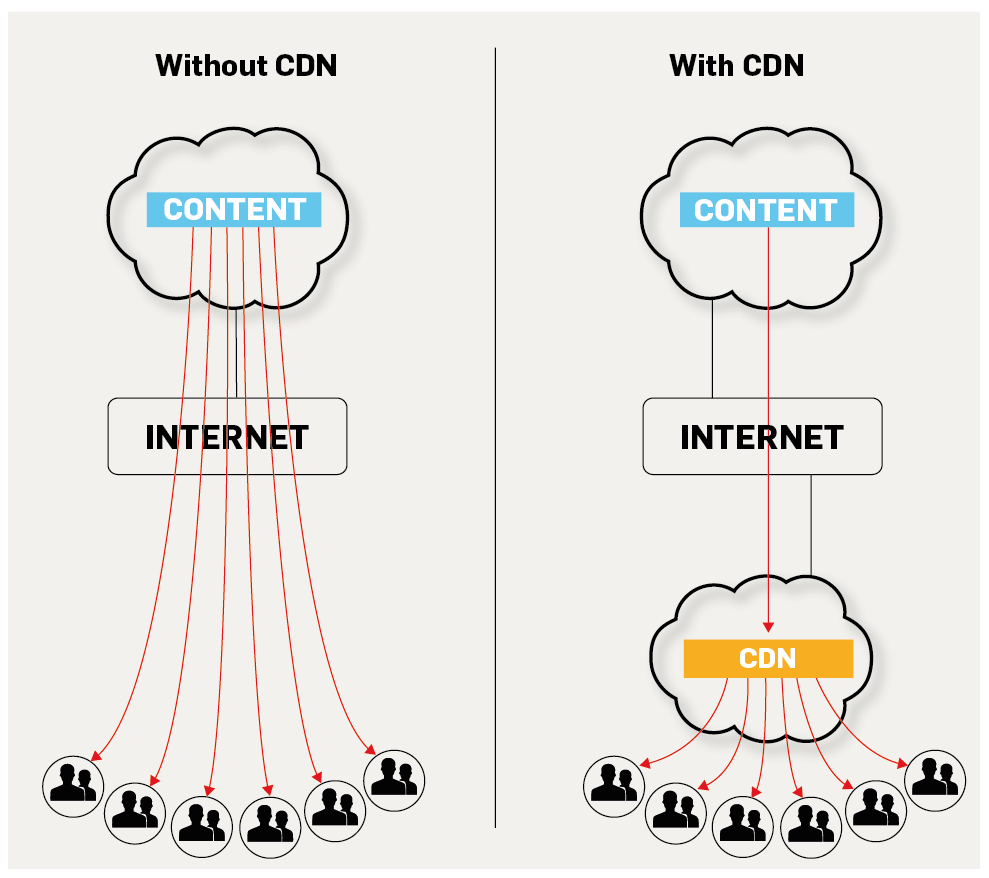
\includegraphics[height=0.6\textheight]{cdn_or_not.png}
    \caption{Caching content closer to demand}
    \end{figure}

\end{frame}

\subsection{Assessing demand satisfaction}
\begin{frame}
    \frametitle{Multicommodity Flow = Content Delivery}

    \begin{center}
    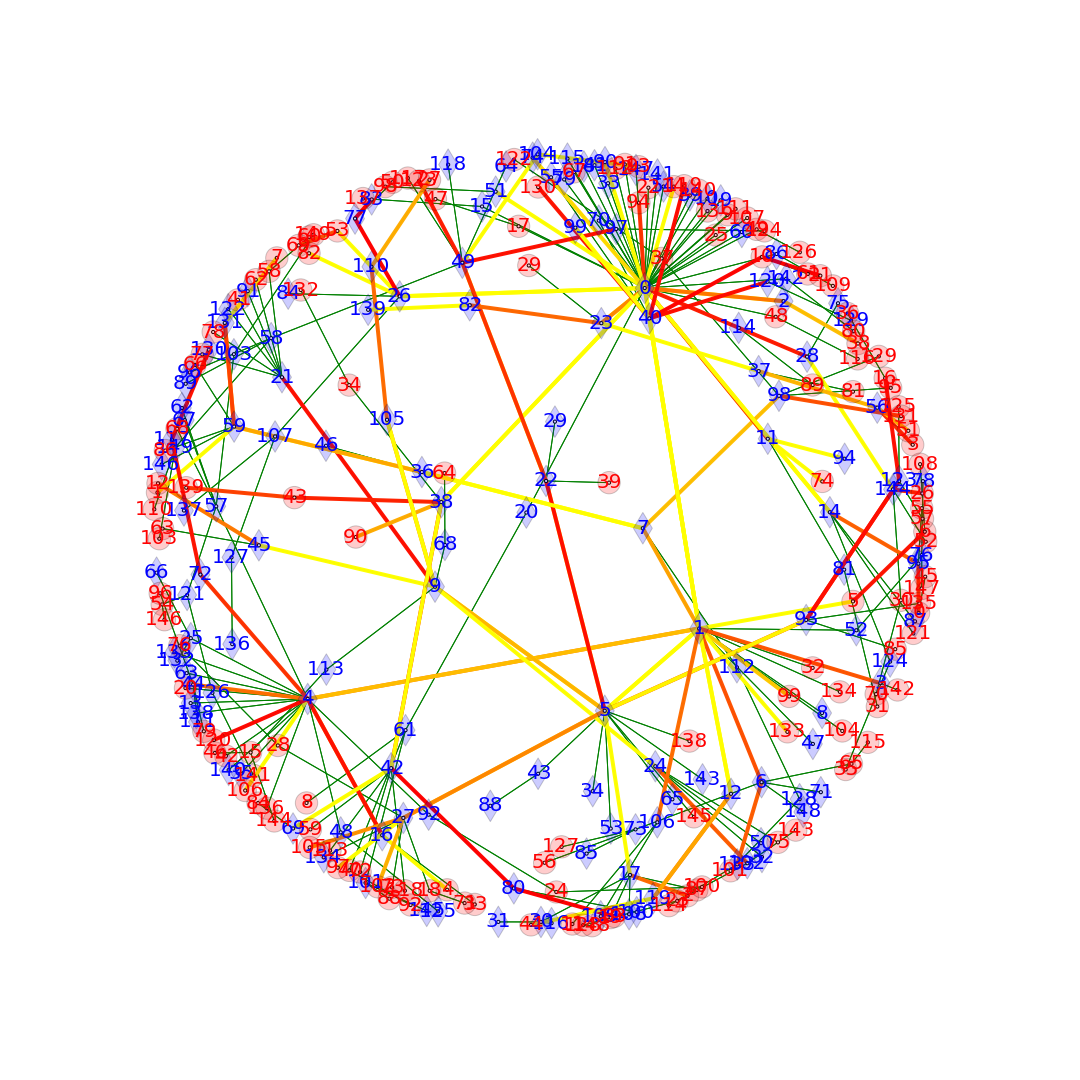
\includegraphics[trim = 20mm 20mm 20mm 20mm, clip, width=0.6\textwidth]{earth.png}

        \begin{tabular}{r | l}
        source & cache server\\
        target & client\\ 
        capacity & bandwidth\\ 
        commodity & content\\
        \end{tabular}
    \end{center}

\end{frame}

\section{Multicommodity Flow}
\subsection{Solving large flow problems}
\begin{frame}
    \frametitle{Fractional Multiflow is in \sc{P}}
    
    No combinatorial algorithm known to solve multiflow.

    \begin{block}{Polynomial-size LP with edge formulation}
    \begin{align*}
        \max & \sum_{s,t \in K} \sum_{a \in \delta^+(s)} f_a^{s,t}\\
        \text{s.t.} & \sum_{s,t \in K} f_a^{s,t} \leq c_a, ~\forall a \in A\\
                    & \sum_{s,t\in K} \sum_{a \in \delta^-(v)} f_a^{s,t} =
                      \sum_{s,t \in K} \sum_{a \in \delta^+(v)} f_a^{s,t},
                      ~ \forall v \in V \setminus \{s,t\}\\
                    & \sum_{a \in \delta^-(s)} f_a^{s,t} = 0,
                      ~ \forall s \in S \\
                    & f\in \mathbb{R}_+^{|A \times K|}
    \end{align*}
    can be solved in polynomial time with an IPM $\implies \textsc{Multiflow}
    \in \textsc{P}$
    \end{block}

\end{frame}

\subsection{Column generation}
\begin{frame}
    \frametitle{Can it be solved on large instances?}

    \begin{block}{Implicit exponential-size path formulation}
    \begin{align*}
    (\Pi) & \begin{dcases}
    \max~ & \sum_{p\in\mathcal{P}} f_p\\
    \text{s.t.}~& \sum_{p\ni a} f_p \leq c_a,~\forall a\in A ~(l_a)\\
    & f \in \mathbb{R}_+^{|\mathcal{P}|}
    \end{dcases}
    \\
    (\Delta) & \begin{dcases}
    \min~ & \sum_{a\in A} c_a l_a\\
    \text{s.t.}~& \sum_{a\in p} l_a \geq 1,~\forall p\in \mathcal{P} ~(f_p)\\
    & l \in \mathbb{R}_+^{|A|}
    \end{dcases}
    \end{align*}
    \end{block}
\end{frame}

\begin{frame}
    \frametitle{Column generation}

        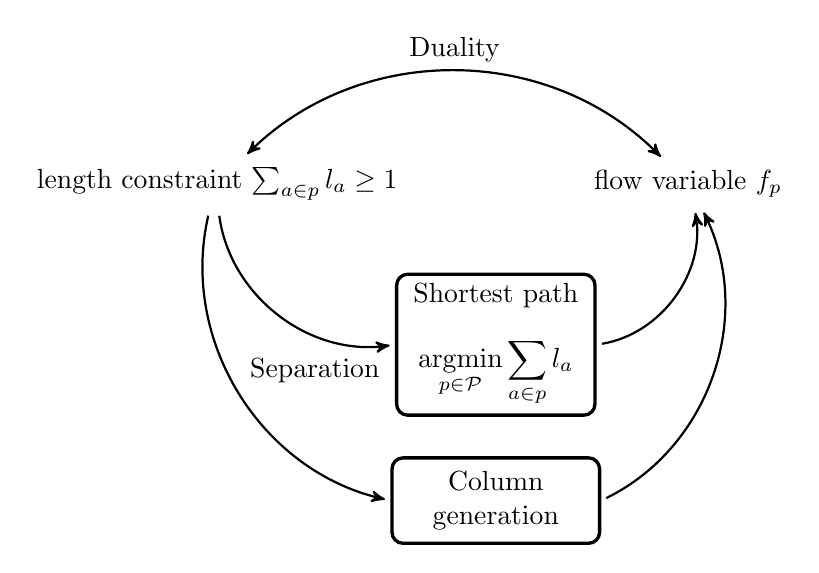
\begin{tikzpicture}[node distance=1cm, auto,]
            \node[punkt]
            (shortestpath)
            {Shortest path
             \begin{equation*}
                \argmin_{p\in \mathcal{P}} \sum_{a\in p} l_a
             \end{equation*}};
            \node[punkt, inner sep=5pt,below=0.5cm of shortestpath]
                (columngen) {Column generation};
                
            \node[above=of shortestpath]
                (dummy) {};
            \node[right=of dummy]
            (t)
            {flow variable $f_p$}
                edge[pil,<-, bend left=45] (shortestpath.east) 
                edge[pil,<-, bend left=45] (columngen.east); 
            \node[left=of dummy]
            (g) {length constraint
                $\sum_{a\in p} l_a \geq 1$
                }
                edge[pil, bend right=45] (shortestpath.west)
                edge[pil, bend right=45] node[midway] {Separation} (columngen.west)
                edge[pil,<->, bend left=45] node[auto] {Duality} (t);
        \end{tikzpicture}

\end{frame}

\subsection{A fast approximation algorithm}
\begin{frame}
    \frametitle{Primal-dual approximation algorithm}

    \begin{block}{Fully Polynomial Time Approximation Scheme}
        An algorithm that returns a solution of value within $\epsilon$ of the
        optimal value:
        \begin{itemize}
            \item in time bounded by a polynomial in the instance size,
            \item in time bounded by a polynomial in $\epsilon^{-1}$.
        \end{itemize}
    \end{block}

    There are combinatorial algorithms that achieve such guarantees.

    \begin{block}{How to design one?}
        \begin{itemize}
            \item leverage the multiplicative weights algorithm
            \item reuse ideas from column generation
        \end{itemize}
    \end{block}

\end{frame}

\begin{frame}
    \frametitle{Multiplicative weights}

    \begin{block}{Background}
        Discovered several times
        \begin{itemize}
            \item 1950's: game theory
            \item 1970's: machine learning
            \item 2000's: design of competitive online algorithms
            \item 2010's: approximation algorithms for SDP
        \end{itemize}
    \end{block}
    \begin{block}{Definition}
        Given a finite set of actions with bounded gain
        \begin{equation*}
            \mathcal{A} = \{ a~|~g_a^t \in [0, 1]  \}
        \end{equation*}

        Associate weights 
        \begin{equation*}
        \forall a\in\mathcal{A}~
        \begin{dcases}
            \lambda_a^{1} &= 1\\
            \lambda_a^{t+1} &= \lambda_a^t (1 + \epsilon~g_a^t)
        \end{dcases}
        \end{equation*}
    \end{block}

\end{frame}

\begin{frame}
    \frametitle{A surprising result}

    \begin{block}{The multiplicative weights algorithm}
        \begin{itemize}
            \item At round $t$, choose action $a$ with probability
                $\dfrac{\lambda_a^t}{\sum_a \lambda_a^t}$
        \end{itemize}
    \end{block}

    \begin{block}{has a guaranteed gain of}
        \begin{equation*}
            G \geq (1 - \epsilon) G_a - \frac{\ln |\mathcal{A}|}{\epsilon},
            ~\forall a \in \mathcal{A}
        \end{equation*}
    \end{block}
    
    \begin{equation*}
    \begin{array}{l l}
        G = \sum_t \mathbb{E}(g^t) & \text{expected gain of the algorithm}\\
        \\
        G_a = \sum_t g^t_a & \text{gain of action $a$}
    \end{array}
    \end{equation*}

\end{frame}

\begin{frame}
    \frametitle{Mapping multiplicative weights concepts to multiflow}

    \begin{block}{Mapping concepts}
    \begin{tabular}{r | c c c | l}
    actions & $\mathcal{A}$ & $\to$ & $A$ & arcs\\
    gain & $g_a$ & $\to$ & $f_a / c_a$ & arc congestion\\
    compound gain & $\lambda_a$ & $\to$ & $l_a$ & length (compound congestion)
    \end{tabular}
    \end{block}

    \begin{block}{Iterative primal-dual algorithm}
        Successively adds flow to the graph
    \end{block}
    
    \begin{block}{Choosing arcs by constraint separation}
        Instead of choosing arcs randomly:
        \begin{itemize}
            \item compute shortest path w.r.t.\ the length $l_a^t$
            \item all arcs on that path receive maximum feasible flow
            \item probabilities are set a posteriori
        \end{itemize}
    \end{block}
\end{frame}

\begin{frame}
    \frametitle{Combining gain guarantee and properties of flows}

    \begin{block}{Using the gain guarantee}
        \begin{equation*}
            G \geq (1 - \epsilon) G_* - \dfrac{\log m}{\epsilon}
        \end{equation*}
        
    \end{block}

    \begin{block}{and simple flow considerations}
        \begin{itemize}
            \item $G_* \begin{dcases} 
                    \text{gain of the best action in hindsight}\\
                    \text{congestion rate of the most congested arc}
                \end{dcases}$
            \item $F / F^* \geq G$: approximation ratio bounds 
                expected gain
        \end{itemize}
    \end{block}

    \begin{block}{results in}
        \begin{itemize}
            \item If $G_* = \log m~\epsilon^{-2}$ then
                $F / G_* \geq (1 - 2\epsilon) F^*$ \alert{$\leftarrow$ AS}
            \item Runtime: $O(km^2\log m~\epsilon^{-2})$ \alert{$\leftarrow$ FPT}
        \end{itemize}
    \end{block}
\end{frame}

\begin{frame}
    \frametitle{Numerical experiments}
    
    \begin{figure}
    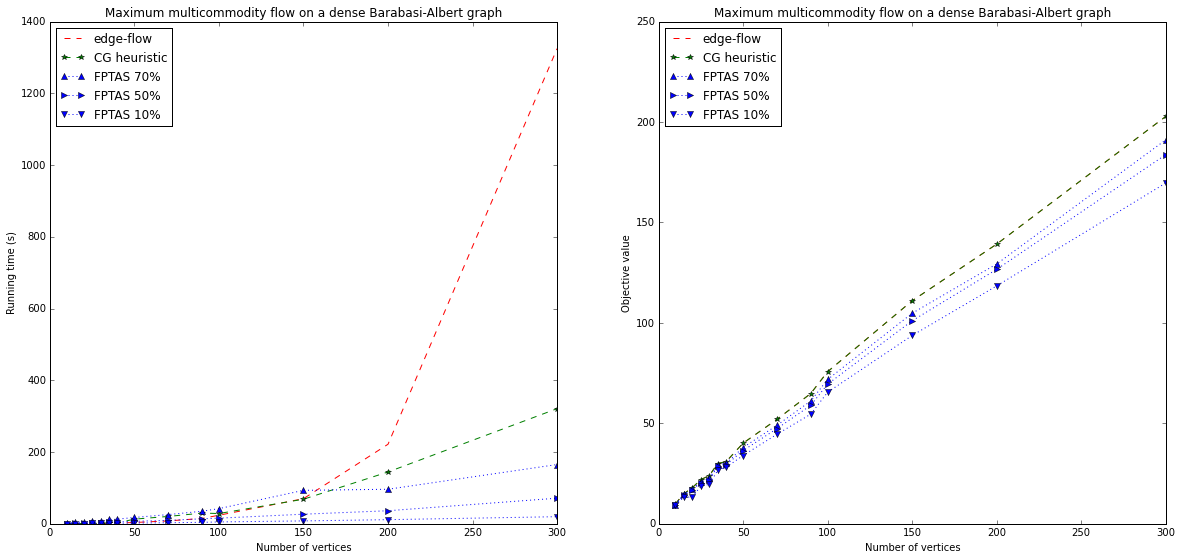
\includegraphics[width=\textwidth]{benchmark_multiflow_ba.png}
    \caption{Performance of LP, column generation, and FPTAS}
    \end{figure}

\end{frame}

\section{Conclusion \& Perspectives}
\begin{frame}
    \frametitle{Conclusion}

    \begin{block}{Highlights}
        \begin{itemize}
            \item CDN design naturally involves multiflows
            \item Approximation: an interesting alternative to exact algorithms
        \end{itemize}
    \end{block}

    \begin{block}{Achievements}
        \begin{itemize}
            \item Studied a theoretical problem in-depth
            \item Implemented a state-of-the-art algorithm
            \item Integrated it in an Operations Research library
        \end{itemize}
    \end{block}

    \begin{block}{Perspectives}
        \begin{itemize}
            \item Studying the matrix multiplicative weights algorithm
            \item Applying it to solve SDP approximatively
        \end{itemize}
        during a PhD at Orange Labs and Universit\'e Paris-Dauphine
    \end{block}
\end{frame}

\begin{frame}
    \frametitle{Thank you!}

    \begin{center}
        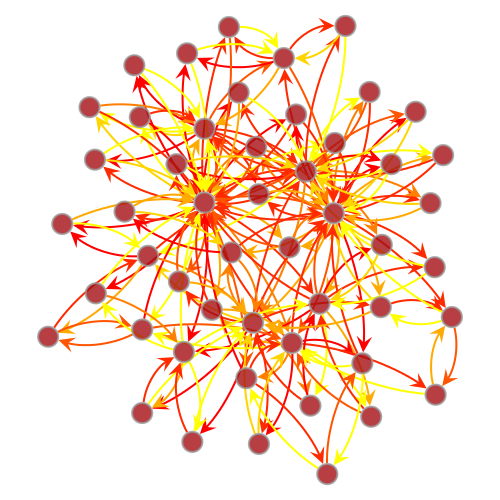
\includegraphics[width=0.5\textwidth]{approx_multiflow.png}

        Any questions?
    \end{center}
\end{frame}

\end{document}
